\chapter{Eksperymenty badawcze}\label{chap:experiments}
Eksperymenty badawcze wyryfikujące charakterystyki sensorów, jak również dokładności opracowanej autorsko hybrydowej metody śledzenia ruchu kończyn, zostały wykonane w~laboratorium technik multimedialnych w~Centrum Technologii Informacyjnych Politechniki Łódzkiej. Jako źródło danych referencyjnych wykorzystany został zainstalowany tam system śledzenia ruchu firmy Vicon zbudowany na bazie 10 kamer Vicon T-40S \cite{ViconSpec} rejestrujących ruch markerów. System ten został skonfigurowany do działania z~częstotliwością 100 klatek na sekundę, a~dane przetwarzane były przez dedykowaną aplikację Nexus w~wersji 2.0. Dane testowe niezbędne do zweryfikowania omawianej metody zostały zgromadzone przy użyciu kontrolera Microsoft Kinect w~wersji dla konsoli XBox 360 model 1414 oraz przez urządzenie rejestrujące dane z~czujników inercyjnych zaprojektowane i~wykonane samodzielnie. Szczegółowy opis przeprowadzonych eksperymentów badawczych znajduje się w~dalszej części niniejszej dysertacji.
%[Fixed] co to znaczy dane dla metody?) zostały zarejestrowane przez 

\section{Scena}
Obszar roboczy, na którym dokonywane były pomiary ruchu, został zamknięty w~przestrzeni (prostopadłościanu) obserwowanej przez kamery systemu Vicon, której obrys podstawy zbliżony był do kwadratu $4m$x$4m$. W~trakcie kalibracji systemu referencyjnego punkt początkowy $\left(0, 0, 0\right)$ został zdefiniowany w~miejscu, w~którym został umieszczony kontroler Kinect.
%([Fixed] niezbędny jest rysunek ze schamtem sceny).  
W~trakcie trwania eksperymentu, badany użytkownik stał w~odległości ok. $2m$ od Kinecta, czyli w~odległości, w~której działa on najbardziej dokładnie.  Pełne rozmieszczenie urządzeń na scenie prezentuje rysunek \ref{fig:experiments:scene}. Prostokąty dookoła obszaru roboczego oznaczone V1 -- V10 to kamery systemu Vicon.
%ten rysunek powinien byc znacznie wcześniej, powinien mieć oznaczone układy współrzednych i~powinno byc od niego odwołanie w~treści pracy
\begin{figure}[!htp]
	\centering
	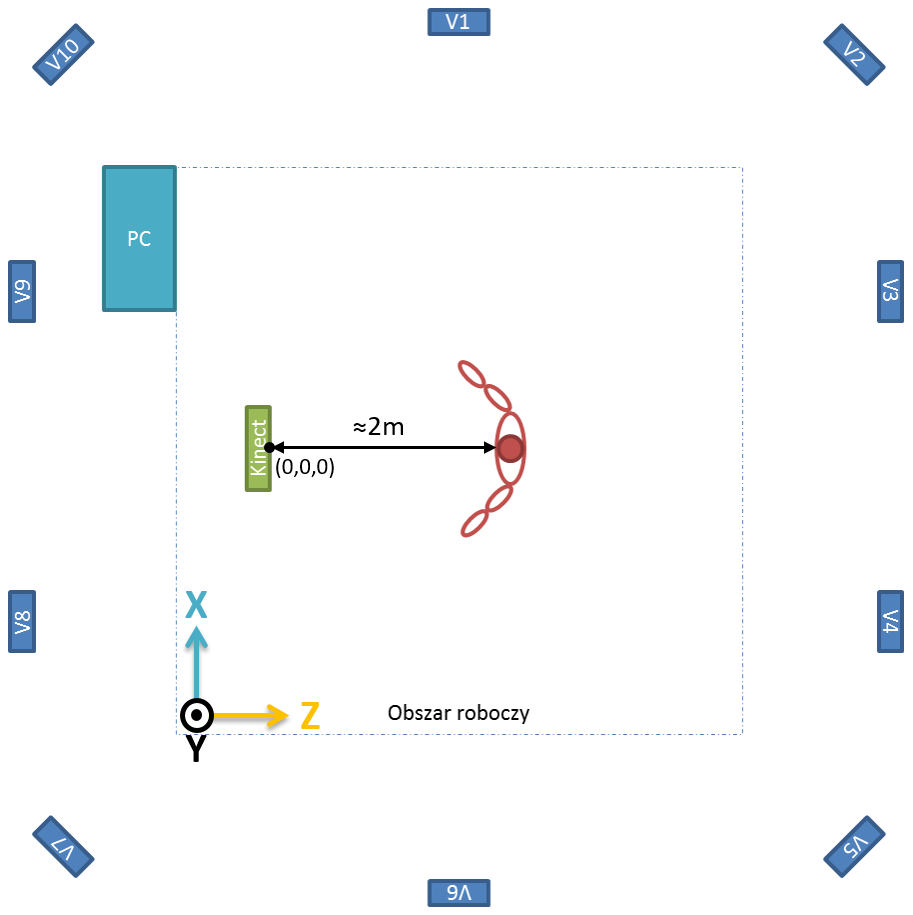
\includegraphics[width=0.7\textwidth]{images/scene.png}
	\caption{Schemat rozmieszczenia elementów sceny w~laboratorium}
	\label{fig:experiments:scene}
\end{figure}
  
 
Eksperymenty badawcze, opisane w~niniejszej pracy, zostały przeprowadzone na przykładzie ruchu ręki, a~oszacowaniu położenia w~przestrzeni podlegały stawy łokciowy oraz nadgarstkowy prawej ręki.
%([Fixed] ale w~eksperymentach biorą udział 2 ręce?)
Jednak nie ogranicza to możliwości zastosowania opracowanej w~pracy metody do śledzenia pozostałych kończyn. Markery niezbędne do prawidłowego działania systemu śledzenia ruchu firmy Vicon zostały umieszczone według schematu zamieszczonego na rysunku \ref{fig:experiments:viconArm}

\begin{figure}[!htp]
	\centering
	\includegraphics[width=0.6\textwidth]{images/Fig11.png}
	\caption{Schemat romieszczenia markerów na ręce zgodny z~zaleceniami systemu Vicon}
	\label{fig:experiments:viconArm}
\end{figure}

Sposób umieszczenia markerów został zaczerpnięty ze schematu ich rozmieszczenia zawartego w~instrukcji do systemu Vicon, jednak poszerzony został o~dodatkowe markery tak, aby nadgarstek i~łokieć śledzony był za pomocą 4 znaczników a~ramię za pomocą 3. Aby móc skutecznie porównać ze sobą położenie stawów, wyznaczonych na podstawie pomiarów z~kontrolera Kinect i~z czujników inercyjnych z~tymi wyznaczonymi przez system śledzenia ruchu Vicon, współrzędne śledzonych markerów, reprezentujące wybrany staw, muszą być uśrednione, tak żeby na ich podstawie obliczyć współrzędne stawów analizowanej kończyny. Do dokładnego wyznaczenia pojedynczego punktu reprezentującego staw, pomocne jest 
%([Fixed] mam wątpliwości czy faktycznie jest niezbędny czy tylko pomocny, bo przecież da się obliczyć na bazie 1 punktu zakładając pewien model biomechaniczny??) 
oszacowanie położenia 3 markerów. Dzięki zastosowaniu uzupełniających markerów do układu rekomendowanego przez firmę Vicon, udało się znacznie ograniczyć liczbę pomiarów, na których były widoczne mniej niż 3 markery, przez co precyzja śledzenia ruchu kończyn była większa. System śledzenia ruchu Vicon, w~wykorzystanej konfiguracji, dostarczał pomiary co 10 ms tj. działał z~częstotliwością 100 Hz.  \\ 
%([NotFixed] można coś wspomnieć o~ksiązkowej dokładności tego systemu i~że może pracować z~wieksza częstotliwością tylko że nie jest to potrzebne) -- nie znalazłem nigdzie dokładności dla tego konkretnego modelu kamer\\

Oprócz markerów niezbędnych dla poprawnego działania systemu Vicon na przedramieniu i~ramieniu, w~połowie ich długości, zostały umieszczone czujniki inercyjne. Czujniki te, aby możliwie wiernie rejestrowały ruchy kończyn zostały przymocowane do skóry za pomocą taśmy klejącej oraz dodatkowo dociśnięte elastycznymi opaskami. Dzięki temu były one w~stanie wykonywać obroty wraz z~kończynami. Zostały one umieszczone na wierzchniej stronie ręki, tam gdzie jest relatywnie cienka warstwa mięśni i~ścięgien. Dzięki temu czujniki w~większym stopniu reagowały na oroty kości i~były mniej wrażliwe na na pracę otaczających je tkanek (wpływ ruchu m.in. skóry, ścięgień i~mięśni na badanie ruchu kości można znaleźć w~\cite{Sati2016,Reinschmidt2016}).
%([Fixed] koniecznie trzeba wspomnieć w~którym miejscu kończyny po obwodzie zostały przymocowane. Warto napisać, że powinno się przymocowywać je blisko kości aby praca mięśni nie miała wpływu na przemiszczanie czujnika względem kości. Może jakiaś pozycja literaturowa, która o~tym pisze.)

\section{Badanie ruchu}

Każdy z~ruchów ręki był wykonany przez troje aktorów i~powtórzony 10 razy w~dwóch seriach po 5 powtórzeń. Podzielenie całego ćwiczenia na serie z~mniejszą liczbą powtórzeń związane było z~efektem zmęczenia aktorów, jakie było widoczne wraz z~kolejnymi powtórzeniami. Ćwiczenia jakie należało wykonać zostały dobrane w~taki sposób, aby sprawdzić opisaną metodę zarówno w~sytuacjach, w~których kontroler Kinect i~czujniki inercyjne działają w~uprzywilejowanym dla nich zakresie pracy jak i~w~takich, w~których jedno z~urządzeń posiada istotne ograniczenia w~działaniu. Wszystkie sekwencje rozpoczynały się od pozycji wyjściowej z~rękami rozłożonymi na boki tzw. \emph{T--pose}. Następnie, wykonywano zgięcie rąk w~łokciu ku górze i~ich wyprostowanie w~celu zsynchronizowania pomiarów Kinecta i~czujników inercyjnych w~czasie. Po sekwencji synchronizującej następowały właściwe ćwiczenia, w~których każde powtórzenie zaczynało i~kończyło się pozycją \emph{T--pose}. Wykonywane ćwiczenia prezentuje rysunek \ref{fig:experiments:poses}

\begin{figure}[!htp]
	\centering
	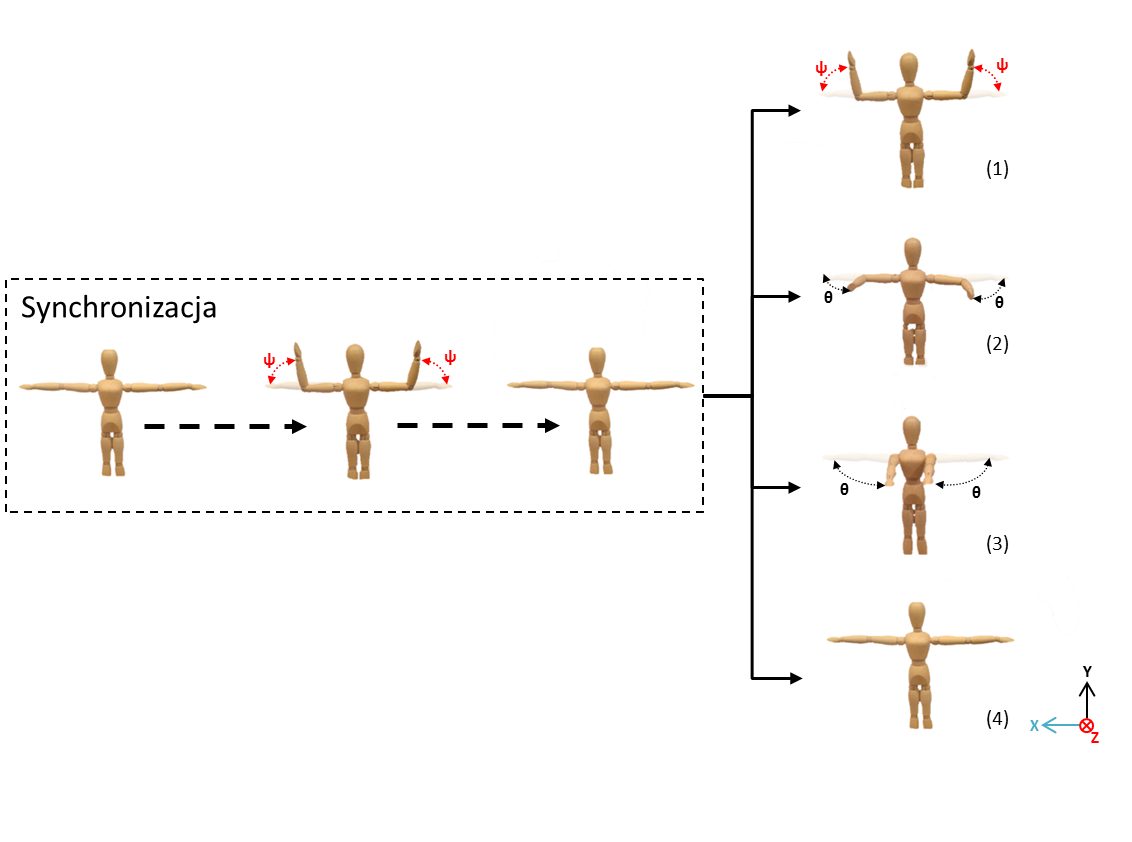
\includegraphics[width=\textwidth]{images/poses.png}
	\caption{Ćwiczenia wykonywane w~ramach eksperymentu}
	\label{fig:experiments:poses}
\end{figure}

W kolejności wykonywane ćwiczenia to:
\begin{enumerate}
	\item Zgięcie ręki w~łokciu do góry; \\
	\item Zgięcie ręki w~łokciu do przodu; \\
	\item Wyciągnięcie wyprostowanych ramion do przodu; \\
	\item Utrzymanie wyprostowanych ramion w~bezruchu przez czas około 60s; \\
\end{enumerate}

Ćwiczenie 1 wykonywane było w~płaszczyźnie, w~której czujniki inercyjne są w~stanie dokonywać dokładnych i~stabilnych w~czasie pomiarów, natomiast dla Kinecta nie następuje okluzja stawów. Ćwiczenia 2 i~3 wymagają wykonania ruchu w~płaszczyźnie, w~której pomiary czujników inercyjnych są błędne i~nie mogą być traktowane jako wiarygodne. Dodatkowo, w~trakcie wykonywania ćwiczenia, kontroler Kinect traci możliwość obserwacji stawów ręki z~powodu ich przesłaniania się. Ostatnie ćwiczenie z~kolei sprawdza stabilność pomiaru w~bez ruchu, który obarczony jest dryfem pomiarów ze strony akcelerometru i~żyroskopu.\\

Wszystkie pomiary zostały porównane z~pomiarami referencyjnymi zarejestrowanymi w~systemie Vicon w~celu określenia dokładności wyznaczania pozycji stawów i~kąta zgięcia w~łokciu. Układy współrzędnych systemu śledzenia Vicon i~systemu opartego na autorskiej metodzie śledzenia ruchu zostały ujednolicone tak aby można było łatwo określić precyzję szacowania położenia stawów. Jako główny przyjęto układ odniesienia systemu Vicon w~którym punkt początkowy $(0,0,0)$ znajdował się na podłodze dokładnie pod kontrolerem Kinect.\\
%([Fixed] dlaczego układ Kinecta był wiodący a~nie ukłąd Vicona? Vicon wydaje się bardziej stabilny.) -- racja, w~kodzie mam jak byk "sprowadzenie Kinecta" do Vicona 
Błąd estymacji pozycji stawów w~pojedynczej sesji wykonywanego ruchu został zdefiniowany jako pierwiastek kwadratowy z~błędu średniokwadratowego (RMSE) odległości ($d_e$) pomiędzy referencyjną pozycją danego stawu zmierzoną w~systemie Vicon $P^V_j$, a~pozycją oszacowaną ($P^F_j$) i~jest wyrażony wzorem \eqref{eq:experiments:RMSE}. Następnie została obliczona średnia arytmetyczna z~wyznaczonych RMSE w~celu wyznaczenia dokładności szacowania pozycji stawów w~każdym z~wykonanych ćwiczeń. Podobną metodologię określania błędu oszacowania badanej metody zastosowani w~swoich pracach m.in. Kassim et al. \cite{Kassim2008} oraz Tadano et al. \cite{Tadano2013}. W~analogiczny sposób został także oszacowany błąd wyznaczania kąta zgięcia stawu łokciowego $\beta$.

\begin{equation}
	\centering
	RMSE^F_j = \sqrt{\frac{1}{n}\sum_{i=1}^{n}{d_e(P^V_{j,i}, P^F_{j,i})^2}}
	\label{eq:experiments:RMSE}
\end{equation}

%([Fixed] co to jest średnia z~porównań pomiarów?? Może trzeba napisać co było uśredniane i~dlaczego i~co było porównywane?). 
Powyższe błędy szacowania pozycji stawów oraz kąta zgięcia stawu łokciowego zostały wyznaczone dla opisywanej w~niniejszej dysertacji metodzie łączenia danych opartej na obrotach kości ($P^{F,O}_j$,$\beta^{F,O}$) oraz dla analogicznych oszacowań uzyskanych za pomocą metody o~najniższym opisanym w~literaturze błędzie szacowania położenia stawów, opierającej się na łączeniu danych o~pozycjach poszczególnych stawów tj. metodą zaproponowaną przez Kalkbrenner et al. \cite{Kalkbrenner2014}.(nazywana dalej metodą Kalkbrennera, $P^{F,P}_j$,$\beta^{F,P}$)\\

%[Fixed]trzeba wprowadzic pojęcie średniej dokładności, które następnie pojawi się analizie. Nie wiadomo dokładnie z~tekstu jak średnie odległości przekładają się na dokładność szacowania pozycji. Ta dyskusja już była: czy szacujemy błąd, czy szacujemy dokładność, czy może coś jeszcze?
Każda z~sesji śledzenia konkretnego ruchu składała się z~5 nieprzerywanych powtórzeń tego samego ruchu. Dla każdej z~takich sesji zostały wyliczone wartości RMSE każdego z~wyżej wymienionych oszacowań (pozycje stawów łokciowego ($P^F_E$) i~nadgarstkowego ($P^F_W$) oraz kąt zgięcia łokcia $\beta^F$). Całkowity błąd szacowania metody został określony jako średnia arytmetyczna $\overline{RMSE}$ ze wszystkich sesji śledzenia ruchu dla danego stawu lub kąta $\beta$.

Wyniki zostały zebrane w~tabelach \ref{tab:experiments:first:avg}, \ref{tab:experiments:sec:avg}, \ref{tab:experiments:thr:avg} i~\ref{tab:experiments:four:avg}.

%([Fixed] tzn jak 5 powtórzeń jest brane pod uwagę gdy obliczane sa wyniki. Co jest uśredniane, kiedy i~jak?)

Porównanie pomiędzy wynikami uzyskanymi za pomocą metody Kalkbrennera i~metody łączenia danych opartej na obrotach kości zostało wyznaczone jako stosunek różnicy pomiędzy uśrednionym RMSE dla metody Kalkbrennera ($\overline{RMSE^P_j}$) a~uśrednonym RMSE dla metody opracowanej przez autora niniejszej dysertacji ($\overline{RMSE^O_j}$) do $\overline{RMSE^P_j}$ (wz. \eqref{eq:experiments:comparison}).\\
%([Fixed] średnia dokładność jest pojęciem nie do końca zdefiniowanym)
\begin{equation}
	r = \frac{\overline{RMSE^P_j} - \overline{RMSE^O_j}}{\overline{RMSE^P_j}}
	\label{eq:experiments:comparison}
\end{equation}

%([TODO] w~opisie powyżej nie było żadnej informacji o~modelu biomechanicznym kości, a~przeciez coś było przyjmowane aby można było to wszystko wyliczyć!!!) -- chyba nie rozumiem

\section*{Ćwiczenie 1 -- Zgięcie ramienia w~łokciu do góry}
Pierwsze ćwiczenie, jakie zostało wykonane z~użyciem omawianej metody, to zgięcie ręki w~łokciu do~góry. Jest to ruch łatwy do śledzenia dla obu urządzeń pomiarowych ze względu na brak występowania okluzji stawów oraz prostopadłej do wektora grawitacji płaszczyźnie wykonywania ruchu. Wyniki uzyskane w~tym ćwiczeniu prezentuje tabela \ref{tab:experiments:first:avg}
%w tabeli pojawia się średnia, ale nie wiemy jaka to średnia. W~wierszach jest 6 pozycji więc nie wiemy skąd 6 skoro były 2 serie po 5 ?? Jak się mają wartości w~wierszach do wspólczynników i~parametrów, które sa liczone powyżej (r, średnia dokładność, średni błąd) ? Trochę jest w~tym bałagan.
\begin{table}[!htp]
	\caption{Średni błąd szacowania $\overline{RMSE}$  dla ćwiczenia nr 1}
	\label{tab:experiments:first:avg}
	\noindent
	\tiny
	\centering
	\begin{tabular}{|c|c|c|c|c|c|c|}
		\hline 
		& \multicolumn{3}{c|}{Metoda autorska} & \multicolumn{3}{c|}{Metoda Kalkbrennera}  \\ 
		\hline 
		Sesja                      & $RMSE^O_E$ & $RMSE^O_W$ & $RMSE^O_\beta$ & $RMSE^P_E$ & $RMSE^P_W$ & $RMSE^P_\beta$ \\
		śledzenia                 & $[cm]$     & $[cm]$     & $[\degree]$    & $[cm]$     & $[cm]$     & $[\degree]$    \\
		\hline
		1                          & 2.2        & 2.7        & 3.24           & 2.6        & 3.1        & 3.44           \\
		2                          & 2.3        & 2.8        & 3.33           & 2.7        & 3.1        & 3.77           \\
		3                          & 2.2        & 2.7        & 3.15           & 2.5        & 3.0        & 3.42           \\
		4                          & 2.3        & 2.7        & 3.18           & 2.6        & 3.0        & 3.48           \\
		5                          & 2.1        & 2.8        & 3.35           & 2.5        & 2.9        & 3.51           \\
		6                          & 2.3        & 2.8        & 3.52           & 2.6        & 3.0        & 3.63           \\
		\hline
		Średnia $\overline{RMSE}$ & 2.2        & 2.8        & 3.30           & 2.6        & 3.0        & 3.542          \\
		Odchylenie                 & 0.08       & 0.05       & 0.12           & 0.07       & 0.07       & 0.12           \\
		\hline
	\end{tabular} 
								
\end{table} 

Ćwiczenie polegające na wielokrotnym zgięciu ręki w~łokciu do góry, zgodnie z~przewidywaniami, dla obu urządzeń pomiarowych nie były trudne. Przez cały czas trwania ćwiczenia stawy były poprawnie identyfikowane i~w~pełni śledzone przez kontroler Kinect. Także czujniki inercyjne były w~stanie zarejestrować w~pełni  wykonywany ruch. Także obie porównywane ze sobą metody łączące dane dokonywały zbliżonych obliczeń, a~zakres szacowanego przez nie ruchu był zbliżony do tego wykonywanego na żywo. Widoczne było natomiast zróżnicowanie w~dopasowaniu szkieletu do ciała ze względu na przyjęty model długości kości. W~metodzie Kalkbrennera miała miejsce częsta zmiana tego oszacowania co wpływało na to, że śledzony staw potrafił zmienić swoje położenie bez ruchu, a~także potrafił znaleźć się poza konturem postaci. W~przypadku metody autora niniejszej rozprawy, zauważalne były częste, jednak niewielkie, fluktuacje oszacowania pozycji stawów jednak nie wpływały one na błąd szacowania w~takim stopniu jak zmienna długość segmentów reprezentujących kości. Wydaje się również, że to właśnie brak stałego modelu długości kości w~metodzie Kalkbrennera ma największy wpływ na różnicę uzyskiwanych wyników. \\
%([TODO] pojawia się jedynie analiza pozycji a~co z~czasem?? Brak poza tym dokładnej deklaracji jak w~Twojej metodzie przyjęty jest model kostny.) -- chyba nie bardzo rozumiem

W omawianym ćwiczeniu ruch wykonywany był głównie przez przedramię, czyli istotne i~zamierzone zmiany położenia były widoczne na stawie nadgarstkowym. Wykresy \ref{fig:experiments:first:wristX}, \ref{fig:experiments:first:wristY},\ref{fig:experiments:first:wristZ} pokazują położenie stawu nadgarstkowego w~każdej z~3 osi w~trakcie wykonywania ruchu. Widać na nich wyraźną różnicę w~stabilności pomiarów objawiająca się ciągłymi drganiami widocznymi na wykresie złączenia danych za pomocą metody Kalkbrennera.

%([Fixed] w~poniższych rysunkach trzeba powiększyć teksty opisu, bo sa niewidoczne. Poza tym warto dla dowolnego fragmentu wykresu zastosować coś na zasadzie lupy aby dokładniej zobaczyć jak się mają te wykresy do siebie. Teraz jest trochę mało czytelnie.)
\begin{figure}[!htb]
	\centering
	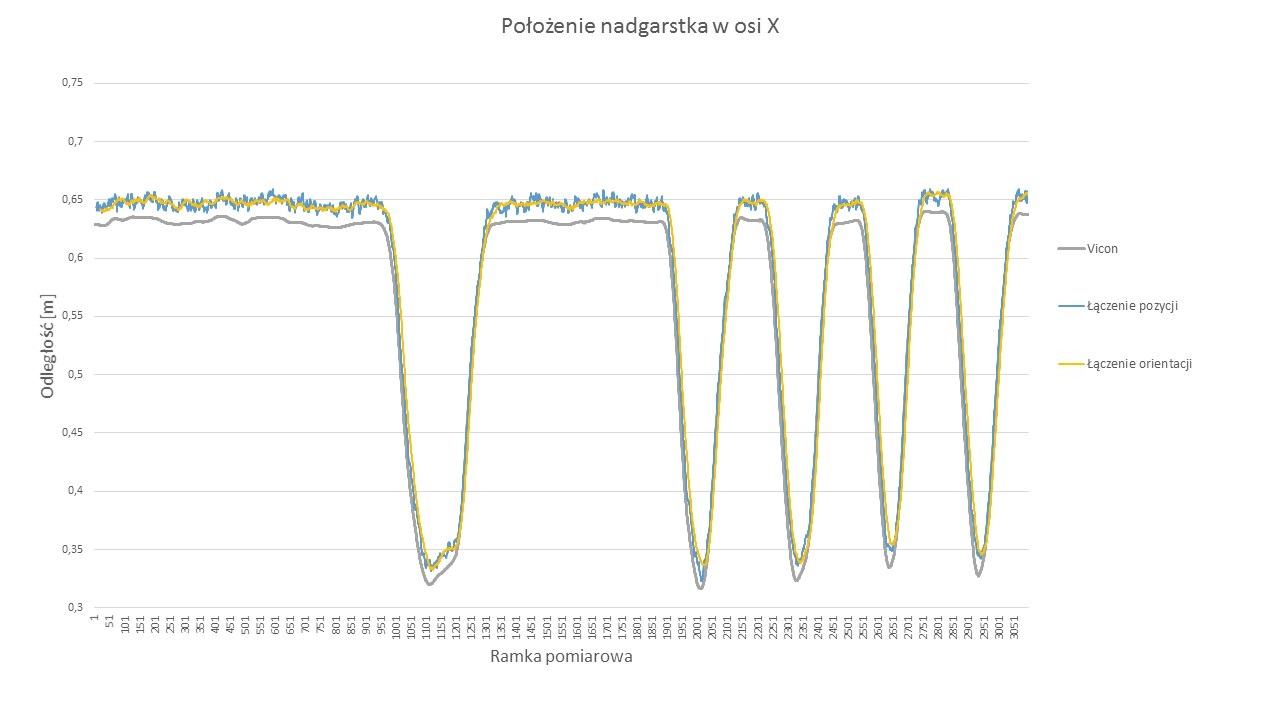
\includegraphics[width=0.9\linewidth]{images/100/Slide4.png}
	\caption{Wykres przedstawiający położenie stawu nadgarstkowego w~osi X}
	\label{fig:experiments:first:wristX}
\end{figure}


\begin{figure}[!htb]
	\centering
	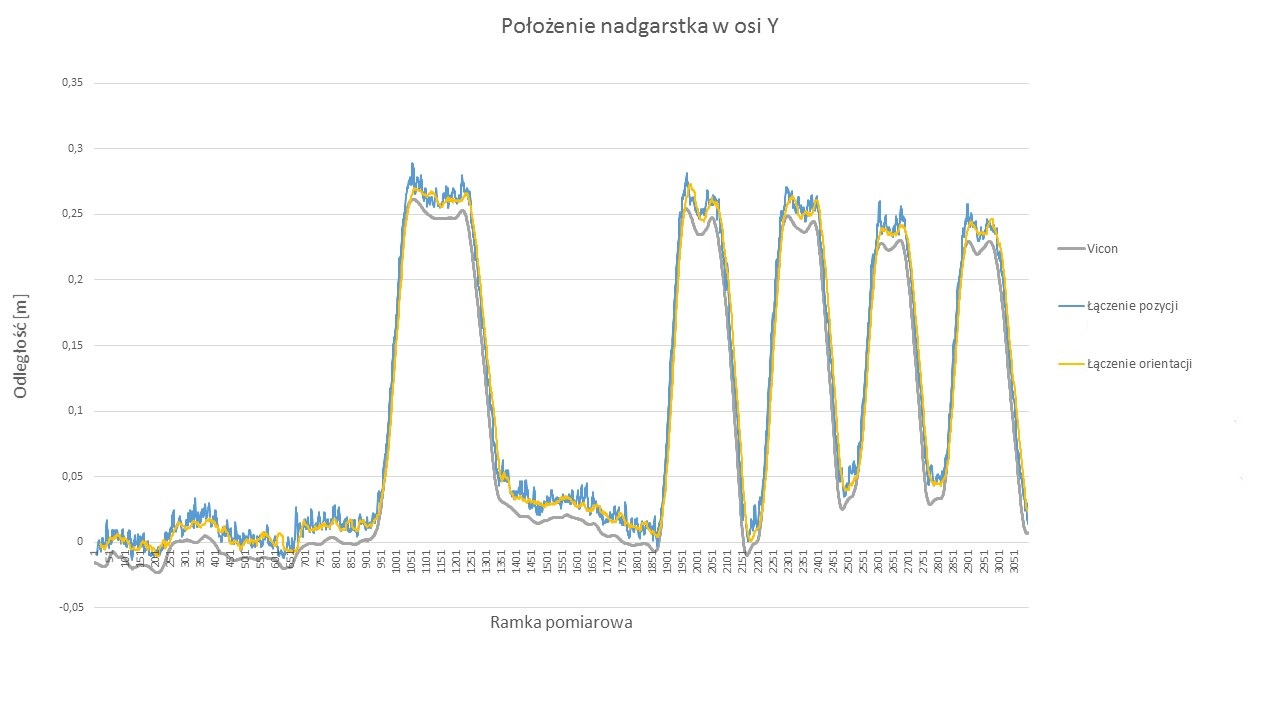
\includegraphics[width=0.9\linewidth]{images/100/Slide5.png}
	\caption{Wykres przedstawiający położenie stawu nadgarstkowego w~osi Y}
	\label{fig:experiments:first:wristY}
\end{figure}

\begin{figure}[!htb]
	\centering
	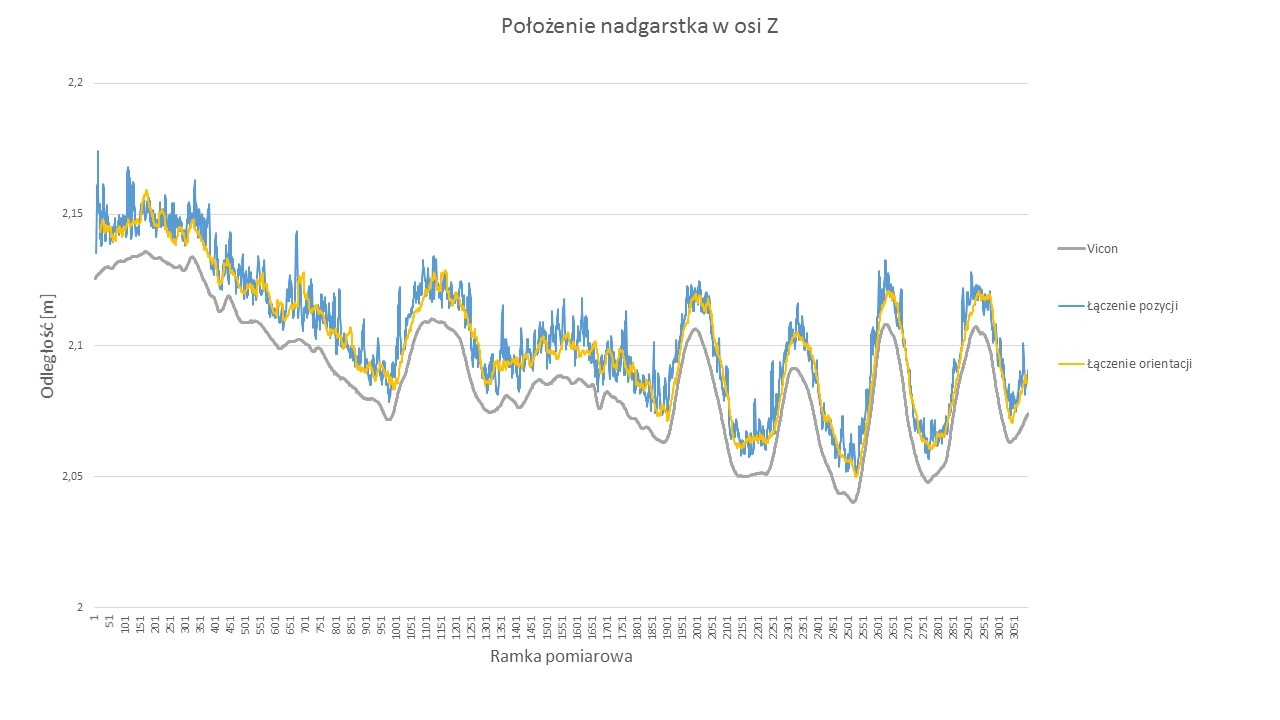
\includegraphics[width=0.9\linewidth]{images/100/Slide6.png}
	\caption{Wykres przedstawiający położenie stawu nadgarstkowego w~osi Z}
	\label{fig:experiments:first:wristZ}
\end{figure}

Rysunki \ref{fig:experiments:first:raw} oraz \ref{fig:experiments:first:fused} pokazują wizualizację ruchu ręki podczas tego ćwiczenia. W~przypadku obu metod łączenia danych widać poprawę pozycjonowania stawów względem danych otrzymanych bezpośrednio z~urządzeń pomiarowych. 

\begin{figure}[!htb]
	\captionsetup{singlelinecheck=off}
	\centering
	\subfigure[Wizualizacja ruchu bezpośrednio z~urządzeń pomiarowych]{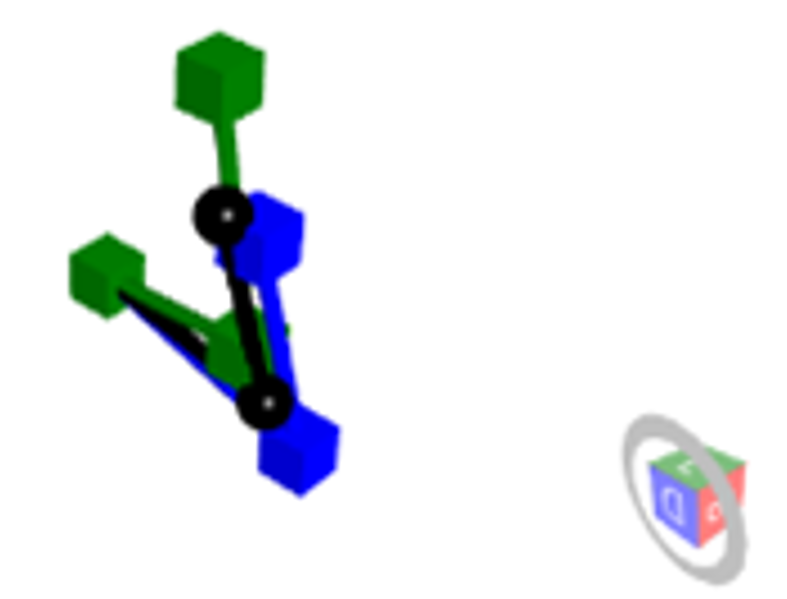
\includegraphics[width=0.45\linewidth]{images/100/raw.png}	\label{fig:experiments:first:raw}}	
	\subfigure[Wizualizacja ruchu po złączeniu danych z~urządzeń pomiarowych]{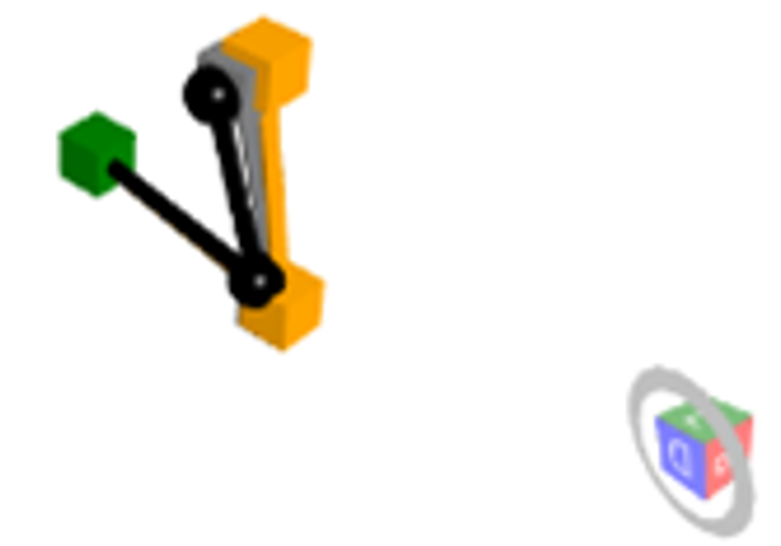
\includegraphics[width=0.45\linewidth]{images/100/Fused.png}		\label{fig:experiments:first:fused}}
	%[Fixed]w podpisie nie robiłbym takiego wypunktowania, tylko wymienił po kolei, bo to źle wygląda. Poza tym na rysunku drugim widać, że Kalkrener jest dokładniejszy niż Twoja metoda, bo jest bliższy Vicona.	
	\caption[Wizualizacja położenia stawów ręki w~ćwiczeniu 1]{Wizualizacja położenia stawów ręki w~ćwiczeniu 1. Kolory: czarny -- Vicon, niebieski -- czujniki inercyjne, zielony -- Kinect, szary -- metoda Kalkbrennera, pomarańczowy -- metoda autorska}	
\end{figure}

\section*{Ćwiczenia 2 i~3 -- Zgięcie ramienia w~łokciu do przodu oraz wyciągnięcie wyprostowanych ramion do przodu}
Ćwiczenia 2 i~3 przedstawiają ruchy o~zwiększonym stopniu trudności śledzenia dla obu urządzeń pomiarowych. W~tym przypadku następuje stopniowe przysłanianie jednego ze stawów co oznacza utratę możliwości dokładnego śledzenia ruchu przez kontroler Kinect. Dodatkowo ruch odbywał się w~płaszczyźnie trudnej z~punktu widzenia czujników inercyjnych, ponieważ obrót dokonywany był wokół osi równoległej do wektora grawitacji. Tabela \ref{tab:experiments:sec:avg} przedstawia średnie dokładności wykonywanego ruchu samego przedramienia, natomiast tabela \ref{tab:experiments:thr:avg} przedstawia wyniki dla ruchu całej wyprostowanej ręki.

%([Fixed] nie zdefiniowano pojęcia średniej dokładności i~teraz to samo zamieszanie co wcześniej. DObrze wprowadzić symbol dla średniej dokładności i~potem go konsekwentnie uzywać w~tabelach i~opisach. SKąd w~tabeli jest 6 wierszy? Z czego to się wzięło?)

\begin{table}[!htp]
	\caption{Średni błąd szacowania $\overline{RMSE}$ dla ćwiczenia nr 2}
	\label{tab:experiments:sec:avg}
	\noindent
	\tiny
	\centering
	\begin{tabular}{|c|c|c|c|c|c|c|}
		\hline 
		& \multicolumn{3}{c|}{Metoda autorska} & \multicolumn{3}{c|}{Metoda Kalkbrennera}  \\ 
		\hline 
		Sesja                      & $RMSE^O_E$ & $RMSE^O_W$ & $RMSE^O_\beta$ & $RMSE^P_E$ & $RMSE^P_W$ & $RMSE^P_\beta$ \\
		śledzenia                 & $[cm]$     & $[cm]$     & $[\degree]$    & $[cm]$     & $[cm]$     & $[\degree]$    \\	
		\hline
		1                          & 2.7        & 3.0        & 14.46          & 3.1        & 3.5        & 15.01          \\
		2                          & 2.5        & 2.8        & 12.72          & 3.1        & 3.0        & 13.07          \\
		4                          & 2.4        & 2.7        & 12.78          & 2.8        & 3.0        & 14.49          \\
		5                          & 2.4        & 2.9        & 13.38          & 3.1        & 3.0        & 15.28          \\
		6                          & 2.5        & 2.9        & 13.41          & 3.2        & 3.0        & 14.61          \\
		\hline
		Średnia $\overline{RMSE}$ & 2.5        & 2.9        & 13.35          & 3.1        & 3.4        & 14.49          \\
		Odchylenie                 & 0.11       & 0.1        & 0.65           & 0.14       & 0.12       & 0.77           \\
		\hline
	\end{tabular} 
								
\end{table} 

\begin{table}[!htp]
	\caption{Średni błąd szacowania $\overline{RMSE}$ dla ćwiczenia nr 3}
	\label{tab:experiments:thr:avg}
	\noindent
	\tiny
	\centering
	\begin{tabular}{|c|c|c|c|c|c|c|}
		\hline 
		& \multicolumn{3}{c|}{Metoda autorska} & \multicolumn{3}{c|}{Metoda Kalkbrennera}  \\ 
		\hline 
		Sesja                      & $RMSE^O_E$ & $RMSE^O_W$ & $RMSE^O_\beta$ & $RMSE^P_E$ & $RMSE^P_W$ & $RMSE^P_\beta$ \\
		śledzenia                 & $[cm]$     & $[cm]$     & $[\degree]$    & $[cm]$     & $[cm]$     & $[\degree]$    \\	
		\hline
		1                          & 2.6        & 3.0        & 13.32          & 3.1        & 3.5        & 15.75          \\
		2                          & 2.2        & 2.5        & 12.37          & 2.9        & 3.3        & 13.12          \\
		3                          & 2.7        & 3.0        & 13.18          & 2.7        & 3.1        & 12.54          \\
		4                          & 2.7        & 3.1        & 14.78          & 3.1        & 3.5        & 16.41          \\
		5                          & 2.2        & 2.6        & 16.77          & 2.7        & 3.0        & 15.75          \\
		\hline
		Średnia $\overline{RMSE}$ & 2.5        & 2.8        & 14.08          & 2.9        & 3.3        & 14.71          \\
		Odchylenie                 & 0.23       & 0.24       & 1.55           & 0.18       & 0.2        & 1.57           \\
		\hline
	\end{tabular} 
								
\end{table} 

W obu ćwiczeniach w~trakcie wykonywania ruchu następował moment, w~którym jeden lub dwa stawy stawały się niewidoczne dla kontrolera Kinect, a~co za tym idzie, obie metody musiały bazować tylko na jednym źródle danych. Metoda opracowana przez autora niniejszej pracy nie wykorzystywała  w~trakcie łączenia danych pomiarów uzyskanych z~niepewnego źródła i~stopniowo wstrzymywała aktualizację estymowanego położenia stawu. Natomiast metoda Kalkbrennera wykorzystywała w~dalszym ciągu dane z~kontrolera Kinect zmieniając jedynie jego stopień istotności (rys. \ref{fig:experiments:sec:follow}). 

Ze względu na to, że kontroler Kinect, pomimo utraty możliwości śledzenia dowolnego stawu, wciąż estymuje jego położenie, zasadne jest sprawdzanie czy fuzja pomiarów dostarczonych przez kontroler Kinect z~pomiarami urządzeń inercyjnych nie sprawi, że ostateczna estymacja położenia stawu stanie się zbyt niedokładna. Metoda Kalkbrennera co prawda dokonuje takiego sprawdzenia w~trakcie stosowania filtru Kalmana, jednak widoczne było podążanie szacunkowych wartości położenia stawu za skokami danych z~Kinecta. Oznacza to, że wpływ pomiarów kontrolera Kinect na ostateczną estymację jest znaczący i~zastosowana w~metodzie Kalkbrennera zmiana stopnia ich istotności w~procesie łączenia danych jest niewystarczająca na ograniczenie negatywnego wpływu niedokładności kontrolera Kinect.
%[Fixed]na pooniższym rysunku totalnie p-omieszałeś kolory dla poszczególnych metod i~czujników. Trzeba to uporządkować. Wszędzie są już takie same: czarny -- Vicon, niebieski -- czujniki inercyjne, zielony -- Kinect, szary -- metoda Kalkbrennera, pomarańczowy -- metoda autorska
\begin{figure}[!htb]
	\centering
	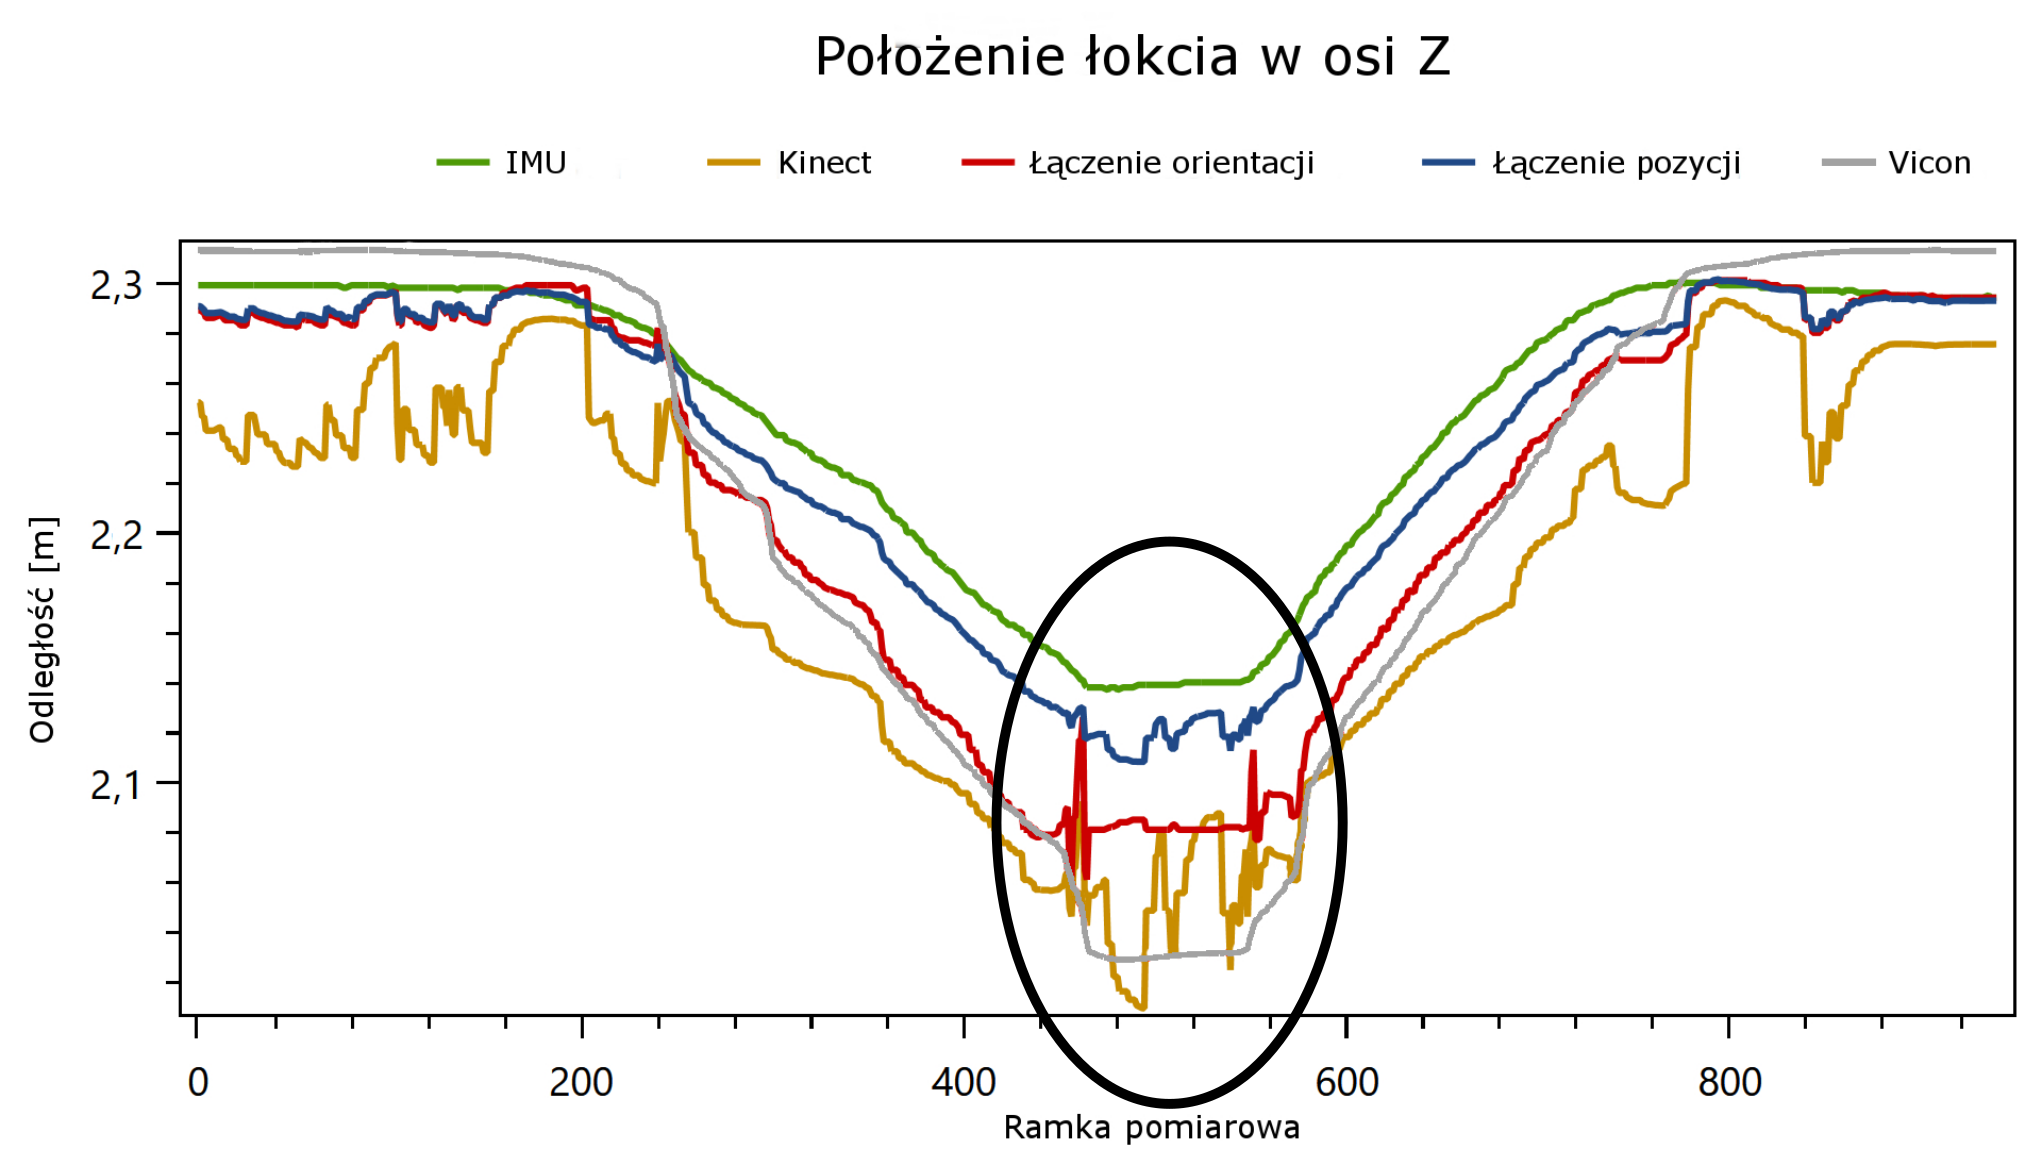
\includegraphics[width=0.8\linewidth]{images/300/Slide3_focus.png}
	\caption{Wykres przedstawiający podążanie wyznaczania pozycji stawu za pomiarami Kinecta w~trakcie wykonywania ćwiczenia 3}
	\label{fig:experiments:sec:follow}
\end{figure}

\begin{figure}[!htb]
	\captionsetup{singlelinecheck=off}
	\centering
	\subfigure[Wizualizacja ruchu bezpośrednio z~urządzeń pomiarowych]{\includegraphics[width=0.45\linewidth]{images/200/raw.png}	\label{fig:experiments:sec:raw}}	
	\subfigure[Wizualizacja ruchu po złączeniu danych z~urządzeń pomiarowych]{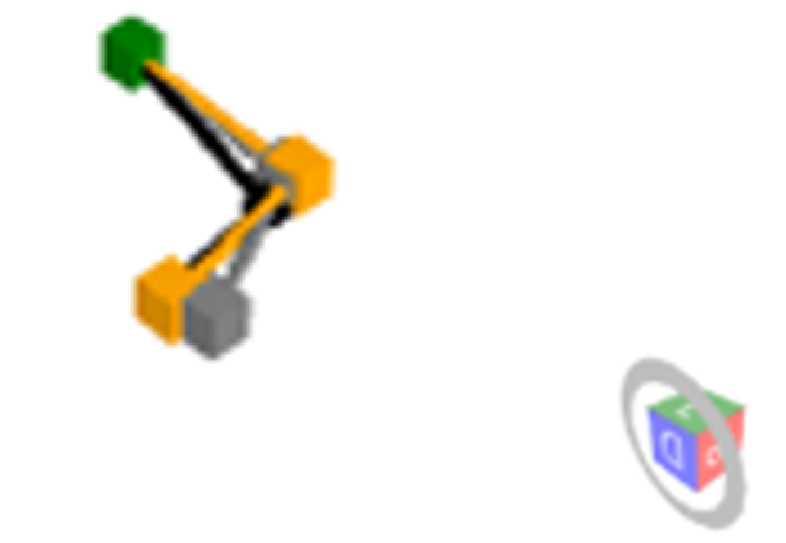
\includegraphics[width=0.45\linewidth]{images/200/Fused.png}		\label{fig:experiments:sec:fused}}	
	\caption[Wizualizacja położenia stawów ręki w~ćwiczeniu 2]{Wizualizacja położenia stawów ręki w~ćwiczeniu 2. Kolory: czarny -- Vicon, niebieski -- czujniki inercyjne, zielony -- Kinect, szary -- metoda Kalkbrennera, pomarańczowy -- metoda autorska}		
	\label{fig:experiments:sec}
\end{figure}
%[Fixed]zlikwidować takie wypunktowanie w~podpisie rysunku. 
\begin{figure}[!htb]
	\captionsetup{singlelinecheck=off}
	\centering
	\subfigure[Wizualizacja ruchu bezpośrednio z~urządzeń pomiarowych]{\includegraphics[width=0.45\linewidth]{images/300/raw.png}	\label{fig:experiments:th:raw}}	
	\subfigure[Wizualizacja ruchu po złączeniu danych z~urządzeń pomiarowych]{\includegraphics[width=0.45\linewidth]{images/300/Fused.png}		\label{fig:experiments:th:fused}}	
	\caption[Wizualizacja położenia stawów ręki w~ćwiczeniu 3]{Wizualizacja położenia stawów ręki w~ćwiczeniu 3. Kolory: czarny -- Vicon, niebieski -- czujniki inercyjne, zielony -- Kinect, szary -- metoda Kalkbrennera, pomarańczowy -- metoda autorska}		
	\label{fig:experiments:th}
\end{figure}

Rysunki \ref{fig:experiments:sec:raw} i~\ref{fig:experiments:th:raw} przedstawiają wizualizację położenia stawów ręki których położenie wyestymowano na podstawie pomiarów uzyskanych bezpośrednio z~urządzeń pomiarowych.
%([Fixed] to zdanie nie ma sensu i~nie wiem jak je poprawić).
Widoczne na nich jest niedokładne szacowanie położenia stawu łokciowego przez kontroler Kinect w~momencie jego przysłonięcia, a~z tym związane jest także niedokładne szacowanie położenia nadgarstka, pomimo jego pełnej widoczności. Widoczne jest także błędne szacowanie obrotu zarówno kości przedramienia jak i~ramienia
%([Fixed] czego?)
wokół osi grawitacji przez urządzenia inercyjne. Wizualizuje to w~pełni ograniczenia w~działaniu obu urządzeń pomiarowych, które zostały opisane w~rozdziale \ref{chap:characteristics}. W~przypadku wizualizacji pozycjonowania stawów łokciowego i~nadgarstkowego 
%([Fixed] czego?)
za pomocą metody Kalkbrennera oraz metody autora niniejszej rozprawy (rys. \ref{fig:experiments:sec:fused} oraz \ref{fig:experiments:th:fused}) w~obu przypadkach widoczne jest zmniejszenie wpływu występowania okluzji stawów jak i~błędów pomiaru obrotu wokół osi grawitacji
%([Fixed] jakich?) 
na ostateczne szacowanie położenia stawów. Widać równocześnie wierniejsze odwzorowanie ruchu w~przypadku metody autora.\\

\section*{Ćwiczenie 4 -- Utrzymanie wyprostowanych ramion}
Celem ostatniego ćwiczenia było sprawdzenie stabilności pomiarów w~przypadku długiego braku ruchu. W~tym wypadku urządzeniem, którego dane pomiarowe mogą szczególnie ulec pogorszeniu w~trakcie działania jest urządzenie zbudowane z~czujników inercyjnych. Tabela \ref{tab:experiments:four:avg} zawiera zestawienie dokładności pomiarów dla tego eksperymentu.

\begin{table}[!htb]
	\caption{Średni błąd szacowania $\overline{RMSE}$ dla ćwiczenia nr 4}
	\label{tab:experiments:four:avg}
	\noindent
	\tiny
	\centering
	\begin{tabular}{|c|c|c|c|c|c|c|}
		\hline 
		& \multicolumn{3}{c|}{Metoda autorska} & \multicolumn{3}{c|}{Metoda Kalkbrennera}  \\ 
		\hline 
		Sesja                      & $RMSE^O_E$ & $RMSE^O_W$ & $RMSE^O_\beta$ & $RMSE^P_E$ & $RMSE^P_W$ & $RMSE^P_\beta$ \\
		śledzenia                 & $[cm]$     & $[cm]$     & $[\degree]$    & $[cm]$     & $[cm]$     & $[\degree]$    \\	
		\hline
		1                          & 2.1        & 2.4        & 4.55           & 2.4        & 2.7        & 4.86           \\
		2                          & 2.3        & 2.6        & 3.86           & 2.4        & 2.7        & 5.10           \\
		3                          & 2.2        & 2.5        & 3.69           & 2.6        & 2.8        & 4.23           \\
		4                          & 2.3        & 2.6        & 4.23           & 2.5        & 2.8        & 4.61           \\
		5                          & 2.6        & 2.5        & 4.32           & 2.4        & 2.7        & 4.84           \\
		6                          & 2.2        & 2.5        & 4.02           & 2.3        & 2.7        & 4.26           \\
		\hline
																		
		Średnia $\overline{RMSE}$ & 2.3        & 2.5        & 4.11           & 2.5        & 2.8        & 4.65           \\
		Odchylenie                 & 0.16       & 0.07       & 0.29           & 0.08       & 0.04       & 0.32           \\
		\hline
	\end{tabular} 
								
\end{table} 

Podobnie jak w~ćwiczeniu 1 tak i~w~ćwiczeniu 4 oba urządzenia były w~stanie przez cały czas trwania eksperymentu śledzić ruchy wykonywane przez śledzonego aktora. Jednak podobnie jak we wspomnianym ćwiczeniu, zmianie ulegały długości segmentów kości i~miało to przełożenie na działanie metody Kalkbrennera. Wizualizacje łańcuchów kinematycznych przedstawione na rysunku \ref{fig:experiments:four} pokazują, że Kinect, mimo pełnej widoczności całej ręki, miał trudność z~poprawnym określeniem jej pozycji w~osi pionowej. Mimo to obie metody były w~stanie wyznaczyć pozycje stawów z~lepszą dokładnością niż każde z~urządzeń pomiarowych osobno.
%[Fixed]zlikwidować brzydkie wypunktowanie w~podpisie do rysunku
\begin{figure}[!htb]
	\captionsetup{singlelinecheck=off}
	\centering
	\subfigure[Wizualizacja ruchu bezpośrednio z~urządzeń pomiarowych]{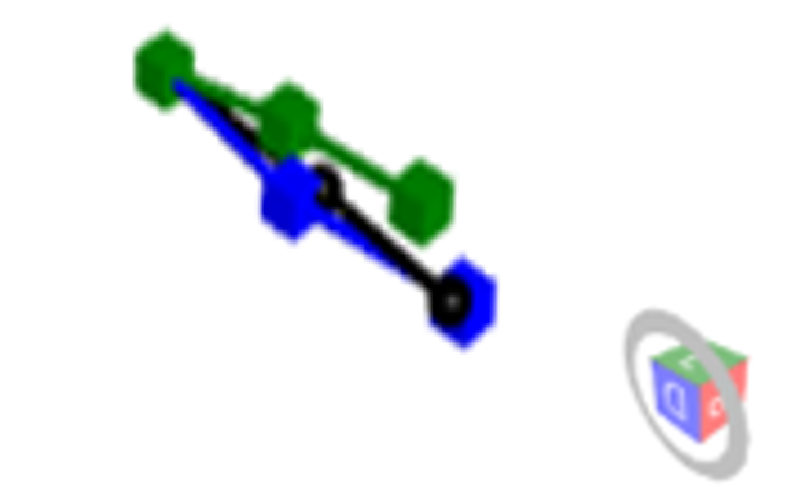
\includegraphics[width=0.45\linewidth]{images/400/raw.png}	\label{fig:experiments:four:raw}}	
	\subfigure[Wizualizacja ruchu po złączeniu danych z~urządzeń pomiarowych]{\includegraphics[width=0.45\linewidth]{images/400/Fused.png}		\label{fig:experiments:four:fused}}	
	\caption[Wizualizacja ruchu ręki w~ćwiczeniu (4)]{Wizualizacja ruchu ręki w~ćwiczeniu (4).  Kolory: czarny -- Vicon, niebieski -- czujniki inercyjne, zielony -- Kinect, szary -- metoda Kalkbrennera, pomarańczowy -- metoda autorska}	
	\label{fig:experiments:four}
\end{figure}

Wykresy estymacji położenia stawów łokciowego (rys. \ref{fig:experiments:four:elbowZ}) oraz nadgarstkowego (rys. \ref{fig:experiments:four:wristZ}) pozwalają zaobserwować wpływ stabilności pomiarów jednego stawu na drugi. Jest to szczególnie widoczne w~wykresie metody Kalkbrennera, gdzie amplituda drgań pozycji nadgarstka jest widocznie większa niż w~przypadku drgań łokcia. 

\begin{figure}[!htb]
	\centering
	\subfigure[Łokieć]{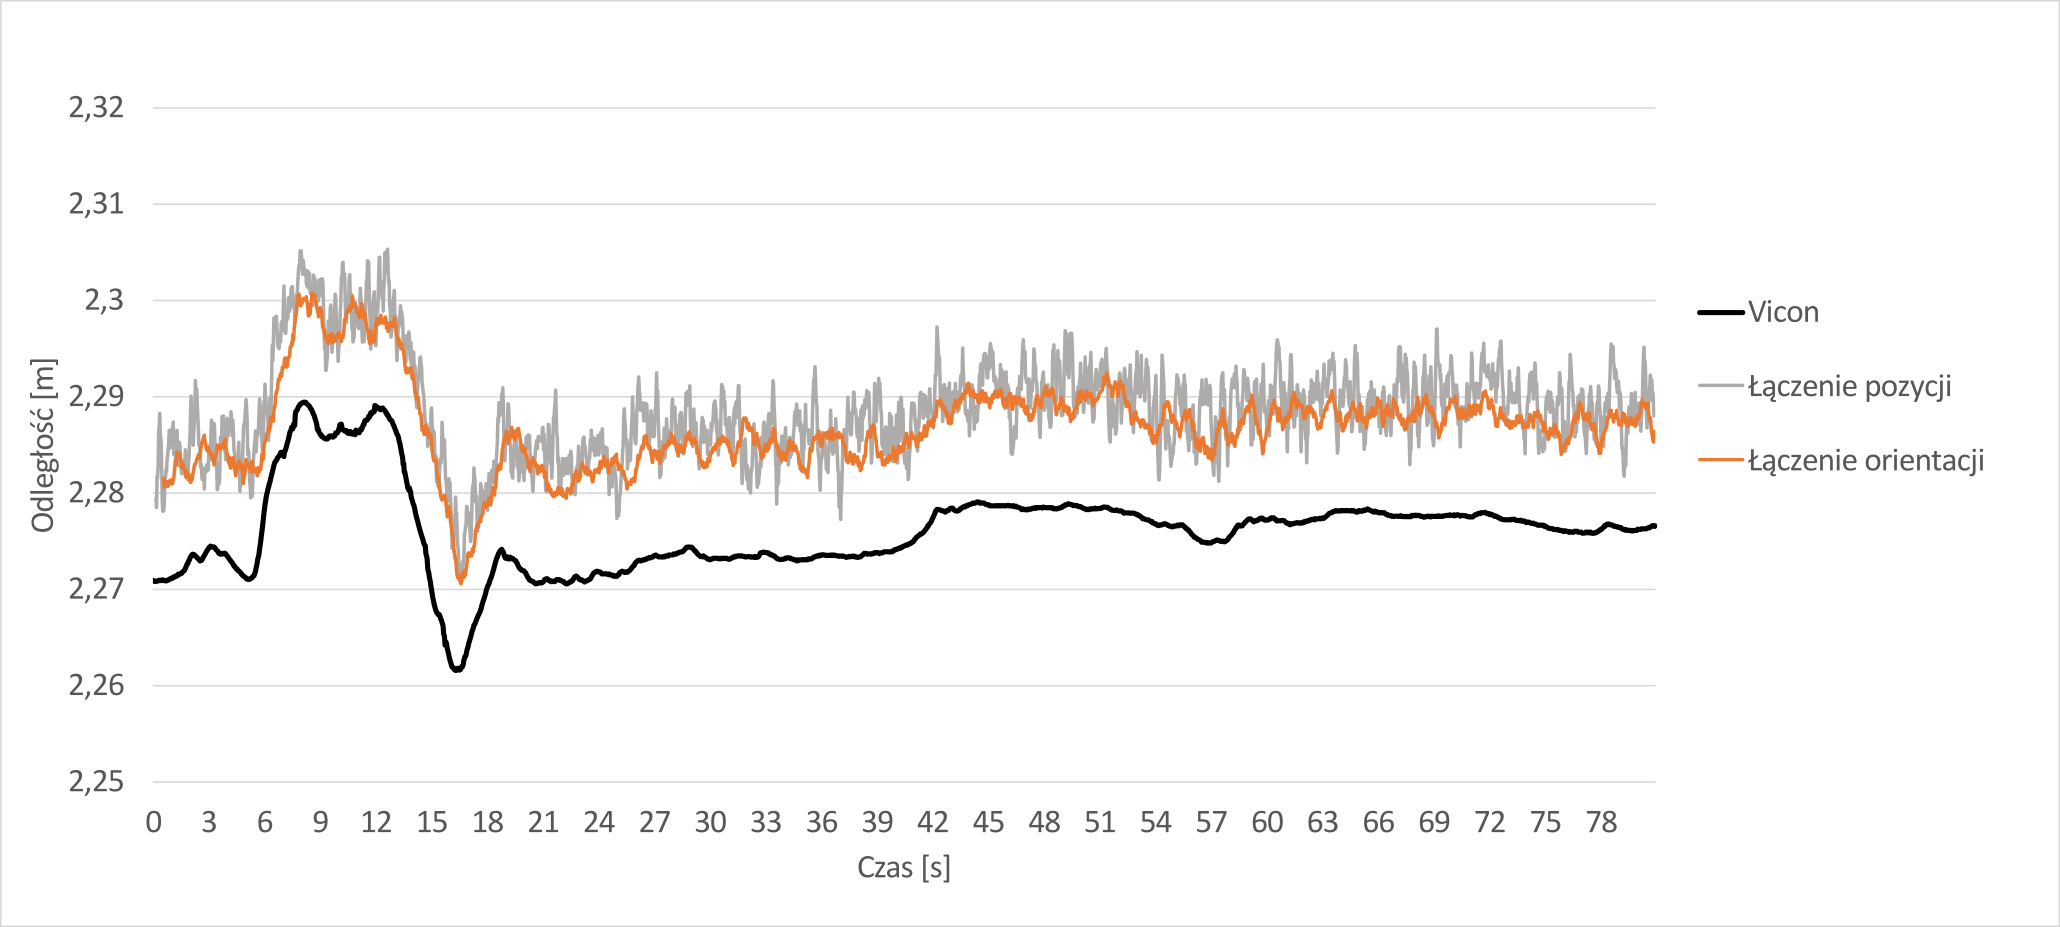
\includegraphics[width=0.45\linewidth]{images/400/3.png}	\label{fig:experiments:four:elbowZ}}	
	\subfigure[Nadgarstek]{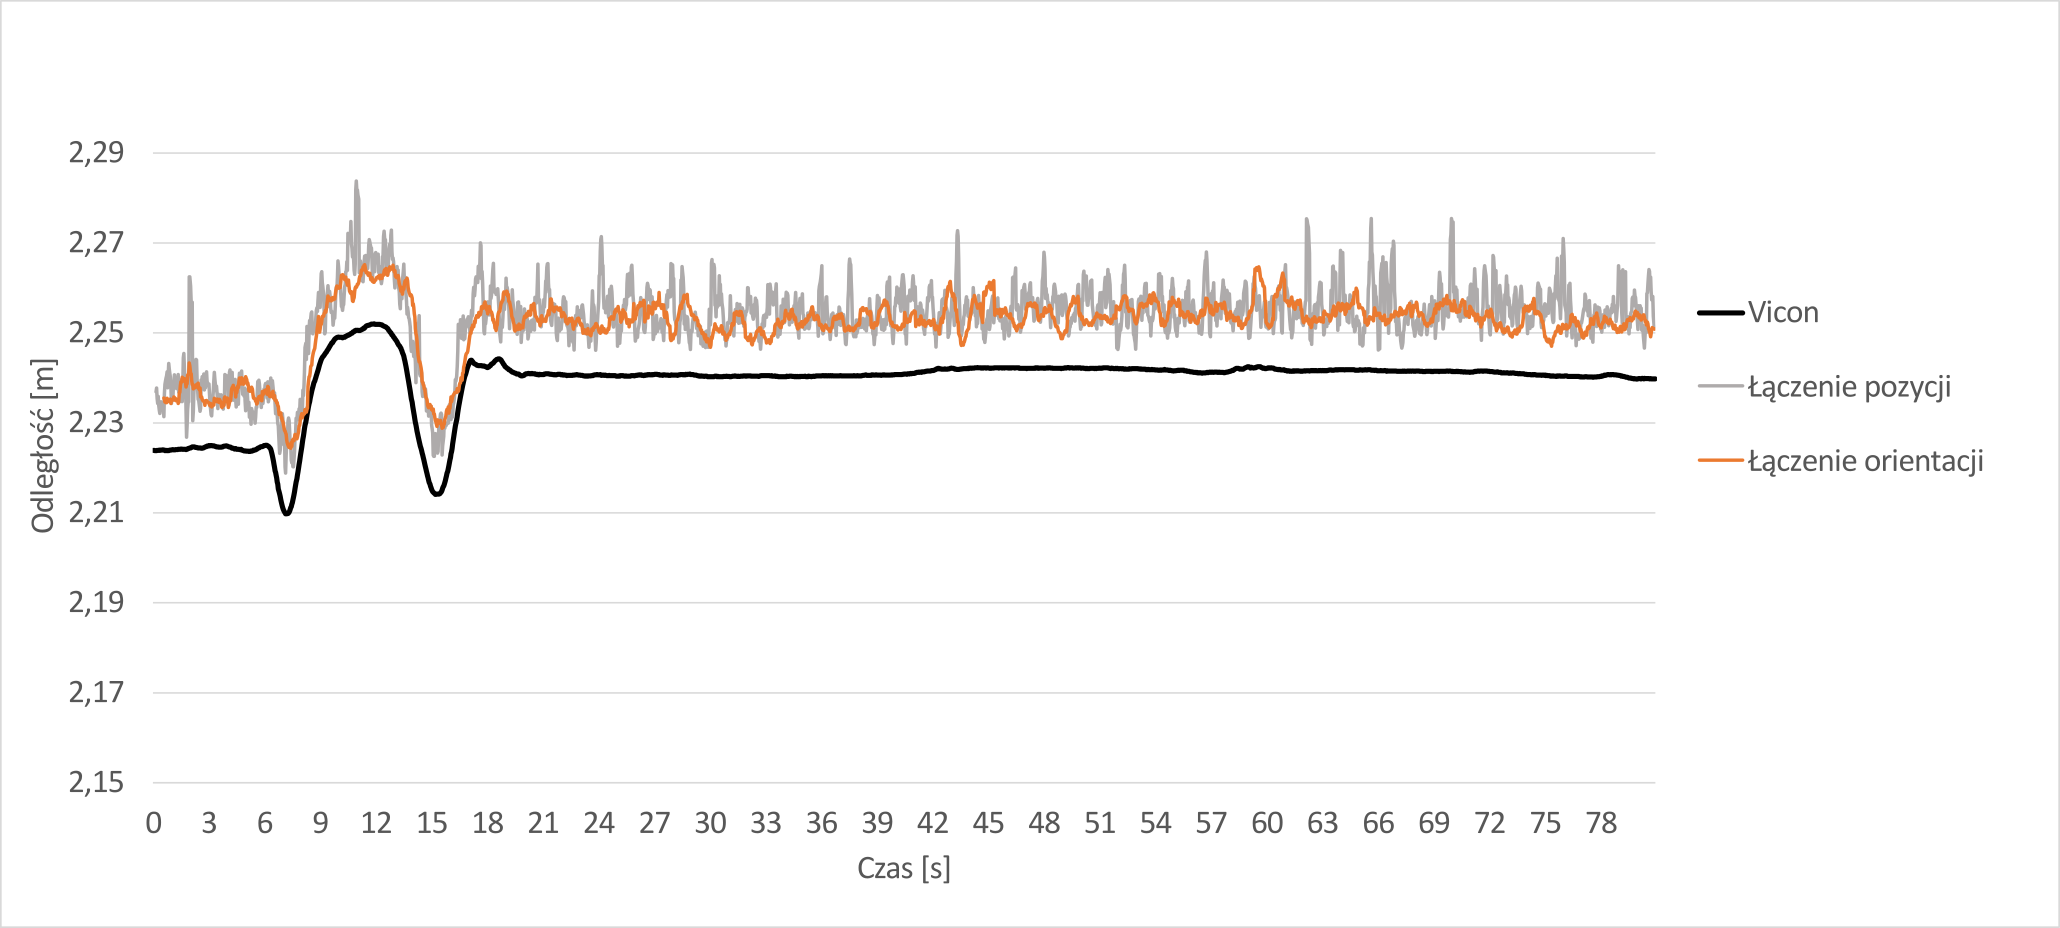
\includegraphics[width=0.45\linewidth]{images/400/6.png} \label{fig:experiments:four:wristZ}}	
	\caption{Wykres położenia stawów w~osi Z~w~ćwiczeniu 4.}	
	\label{fig:experiments:four:Zaxis}
\end{figure}

\section{Podsumowanie}

Ćwiczenia wykonywane w~ramach eksperymentów miały za zadanie sprawdzić działanie metody autora niniejszej pracy, a~także metody Kalkbrennera w~sytuacji, gdy jeden z~czujników przestaje być wiarygodny oraz kiedy dane otrzymywane degradowane są w~czasie. Dla kontrastu weryfikacja dokładności porównywanych metod, dokonana została także na bazie ćwiczenia, które dla obu urządzeń pomiarowych może być nazywane neutralnym (ćwiczenie 1).\\

Porównane ze sobą zostały 3 wartości wyznaczone przez dwie metody mteodę Kalkbrennera i~metodę łączącą dane opartą o~obroty kości. Wartościami porównywanymi pomiędzy obiema metodami były: położenie stawu łokciowego, położenie stawu nadgarstkowego oraz kąt zgięcia ręki w~łokciu. 
%([Fixed] nieprawda bo nie porównujesz stawu łokciwego z~kątem w~łokciu, a~to wynika z~Twojego zdania)
Błąd oszacowania pozycji stawów w~przestrzeni może być wykorzystany jako wskaźnik na ile dana metoda mogłaby być wykorzystana tam gdzie dochodzi do interakcji pomiędzy estymowanym modelem a~otoczeniem. Jako przykład można podać środowisko wirtualne, w~którym znajdują się obiekty którymi można manipulować. Każdy taki obiekt ma swoje ściśle określone położenie w~przestrzeni a~estymacja pozycji stawów jest niezędna żeby określic czy doszło już do "kontaktu" z~takim obiektem czy nie.
 
% Dwie pierwsze wartości pokazują na ile obie metody mogłyby być zastosowane w~systemach śledzenia dla środowisk wirtualnych, gdzie dochodzić może do interakcji z~otoczeniem. ([Fixed] bardzo daleka alegoria, która nie jest zrozumiała. Słabe uzasadnienie zastosowania dla środowisk wirtualnych. Ktoś może nie wiedzieć jak się ma jedno do drugiego, bo nic na ten temat wczesniej nie pisałeś) -- lepiej?
 
Trzecia wartość -- kąt zgięcia ręki w~łokciu -- jest uniezależniona od przyjętych długości kości i~ewentualnych błędów w~pomiarach tych długości. Określa ona wzajemne położenie pomiędzy kością przedramienia a~ramieniem w~zakresie stopnia swobody stawu łokciowego. 
%([Fixed] wszystkie wartości są zależne od przyjętego modelu kości, a~nie tylko ostatnia) 
Ona też pozwala na zweryfikowanie badanych metod śledzenia 
%([Fixed] jakich) 
na potrzeby kontroli zakresu ruchu stawu łokciowego co może być przydatne w~procesie rehabilitacji ruchowej. \\ 
%([Fixed] trochę te zdania mocno wydumane i~pozbawione nalezytego wyjasnienia) -- nie wiem czy teraz lepiej. Generalnei chodzi o~to że kąt oddaje kształt ułożenia ręki i~zakres wykonywanego ruchu a~nie jako taką pozycję przestrznną stawó.

Wykresy z~rysunków \ref{fig:experiments:elbow:summary}, \ref{fig:experiments:wrist:summary} oraz \ref{fig:experiments:angle:summary} pokazują podsumowanie porównania uśrednionych wartości błędu uzyskanych oszacowań ($\overline{RMSE}$)
%([Fixed] znowu nie wiadomo co to jest dokładność uzyskanych wyników)
za pomocą metody Kalkbrennera oraz metody autora tej pracy 
%([TODO] teraz czuje, że metoda powinna mieć jakiś skrót, np. od angielskiej jej nazwy, którą pewnie trzeba wymyśleć - Oriented-based Hybrid Motion Tracking -> OHMT => najbliżej jest MOTH tylko jak? / Jest jeszcze HOMT -> Hybrid, Oriented-based Motion Tracking tylko ten skrótowiec występuje też w~slangu: http://www.urbandictionary.com/define.php?term=H.O.M.T. ). 
Widać na~nich poprawę w~wyznaczaniu położenia stawu łokciowego do 18\%, nadgarstowego do 16\% oraz zdolności szacowania kąta zgięcia ręki w~łokciu do 11\%. Z~przedstawionych wyników wynika większa poprawa w~wyznaczaniu pozycji łokcia niż w~przypadku nadgarstka. Spowodowane jest to kumulowaniem się błędów własnych estymacji położenia nadgarstka, jak i~błędów estymacji położenia łokcia. Jest to cecha charakterystyczna stosowania hierarchicznego modelu ciała człowieka lub jego części. Dla przyjętej hierarchicznej reprezentacji układu kostnego postaci, czym badany staw jest bardziej odległy od punktu początkowego (korzenia) tym dokładność estymacji jego położenia jest mniejsza i~mniejsze są możliwości jej poprawy.\\

Na wykresie z~rysunku \ref{fig:experiments:angle:summary} reprezentującym szacowanie kąta zgięcia ręki w~łokciu widać mniejszą poprawę błedu szacowania pomiędzy obiema badanymi metodami niż miało to miejsce w~przypadku szacowania pozycji stawów. 
%([Fixed] co to jest mniejsza poprawa pomiędzy metodami. To mi jakoś po polsku nie brzmi) 
Na tej podstawie można wyciągnąć wniosek, ze obie porównywane metody: Kalkbrennera oraz autorska w~podobny sposób są w~stanie oszacować wzajemne położenie kości przedramienia i~ramienia. Łącząc to z~wyraźnym zmniejszeniem błędu szacowania pozycji stawów przez metodę opartą na łączeniu obrotów kości i~dodatkowo wykorzystującą (w przeciwieństwie do metody Kalkbrennera) stałą wartość długości kości, można przyjać, że to właśnie przyjęte wartości długości poszczególnych segmentów modelu szkieletowego mają decydujący wpływ na błąd szacowania pozycji stawów. Poprawienie szacowania wartości kąta zgięcia ręki świadczy natomiast o~zmniejszeniu występowania drgań poszczególnych segmentów modelu szkieletowego wyznaczonego przez metodę autora tej pracy.

%([Fixed] znowu trochę nie po polsku, bo na dokładność 2 metod ma wpływ zmiana zastosowana w~jednej metodzie? Nie rozumiem). -- teraz chyba trochę lepiej wytłumaczone.

\pgfplotsset{width=12cm,compat=1.8}
%[fixed]w poniższych rysunkach wprowadzenie w~pionowej osi mdo potęgi -2 są bez sensu. Przeciez to sa centymetry. Nie wiadomo co oznaczają metry/centymetry na pionowej osi
\begin{figure}[!htb]
	\centering
	\begin{tikzpicture}
		\begin{axis}[
				ybar,
				bar width=.5cm,
				width=\textwidth,
				height=.5\textwidth,
				legend style={at={(0.5,1)},
					anchor=north,legend columns=-1},
				symbolic x coords={ex 1,ex 2,ex 3,ex 4},
				xticklabels={Ćwiczenie 1,Ćwiczenie 2,Ćwiczenie 3,Ćwiczenie 4},
				xtick=data,
				ymin=0,ymax=5,
				ylabel={$\overline{RMSE} [cm]$},
			]
			\addplot [black,fill=white,error bars/.cd,y dir=both,y explicit] coordinates { 
				(ex 1,2.6) +- (0.0, 0.07)         
				(ex 2,3.1) +- (0.0, 0.11)
				(ex 3,2.9) +- (0.0, 0.18)  
			(ex 4,2.5) +- (0.0, 0.08) };
			\addplot [black,fill=gray80,error bars/.cd,y dir=both,y explicit] coordinates { 
				(ex 1,2.2) +- (0.0, 0.08)         
				(ex 2,2.5) +- (0.0, 0.14)
				(ex 3,2.5) +- (0.0, 0.23)  
			(ex 4,2.3) +- (0.0, 0.16) };
			\legend{Metoda Kalkbrennera, Metoda autorska}
			\node at (axis cs:ex 1,4){\textcolor{black}{13\%}};
			\node at (axis cs:ex 2,4){\textcolor{black}{18\%}};
			\node at (axis cs:ex 3,4){\textcolor{black}{14\%}};
			\node at (axis cs:ex 4,4){\textcolor{black}{7\%}};
		\end{axis}
	\end{tikzpicture}	
	\caption{Średni błąd $\overline{RMSE}$ wyznaczania pozycji łokcia}
	\label{fig:experiments:elbow:summary}
\end{figure}

\begin{figure}[!htb]
	\centering
	\begin{tikzpicture}
		\begin{axis}[
				ybar,
				bar width=.5cm,
				width=\textwidth,
				height=.5\textwidth,
				legend style={at={(0.5,1)},
					anchor=north,legend columns=-1},
				symbolic x coords={ex 1,ex 2,ex 3,ex 4},
				xtick=data,
				ymin=0,ymax=5,
				xticklabels={Ćwiczenie 1,Ćwiczenie 2,Ćwiczenie 3,Ćwiczenie 4},
				ylabel={$\overline{RMSE} [cm]$},
			]
			\addplot [black,fill=white,error bars/.cd,y dir=both,y explicit] coordinates { 
				(ex 1,3.0) +- (0.0, 0.05)
				(ex 2,3.4) +- (0.0, 0.1)
				(ex 3,3.3) +- (0.0, 0.24)
			(ex 4,2.8) +- (0.0, 0.04)};
			\addplot [black,fill=gray80,error bars/.cd,y dir=both,y explicit] coordinates { 
				(ex 1,2.9) +- (0.0, 0.07)
				(ex 2,2.9) +- (0.0, 0.12)
				(ex 3,2.8) +- (0.0, 0.2)
			(ex 4,2.5) +- (0.0, 0.07)};
																									
			\legend{Metoda Kalkbrennera, Metoda autorska}
			\node at (axis cs:ex 1,4){\textcolor{black}{8\%}};
			\node at (axis cs:ex 2,4){\textcolor{black}{16\%}};
			\node at (axis cs:ex 3,4){\textcolor{black}{14\%}};
			\node at (axis cs:ex 4,4){\textcolor{black}{9\%}};
		\end{axis}
	\end{tikzpicture}
	\caption{Średni błąd $\overline{RMSE}$  wyznaczania pozycji nadgarstka}
	\label{fig:experiments:wrist:summary}
\end{figure}


\begin{figure}[!htb]
	\centering
	\begin{tikzpicture}
		\begin{axis}[
				ybar,
				bar width=.5cm,
				width=\textwidth,
				height=.5\textwidth,
				legend style={at={(0.5,1)},
					anchor=north,legend columns=-1},
				symbolic x coords={ex 1,ex 2,ex 3,ex 4},
				xtick=data,
				xticklabels={Ćwiczenie 1,Ćwiczenie 2,Ćwiczenie 3,Ćwiczenie 4},
				ymin=0,ymax=20,
				ylabel={$\overline{RMSE} [\degree]$},
			]
			\addplot [black,fill=white,error bars/.cd,y dir=both,y explicit] coordinates { 
				(ex 1,3.54) +- (0.0, 0.12)
				(ex 2,14.49) +- (0.0, 0.77)
				(ex 3,14.71) +- (0.0, 1.57)
				(ex 4,4.65)  +- (0.0, 0.32)
			};
			\addplot [black,fill=gray80,error bars/.cd,y dir=both,y explicit] coordinates { 
				(ex 1,3.29) +- (0.0, 0.12)
				(ex 2,13.35)+- (0.0, 0.65)
				(ex 3,14.08)+- (0.0, 1.55)
			(ex 4,4.11)  +- (0.0, 0.29)};
																									
			\legend{Metoda Kalkbrennera, Metoda autorska}
			\node at (axis cs:ex 1,16){\textcolor{black}{6\%}};
			\node at (axis cs:ex 2,16){\textcolor{black}{8\%}};
			\node at (axis cs:ex 3,16){\textcolor{black}{4\%}};
			\node at (axis cs:ex 4,16){\textcolor{black}{11\%}};
		\end{axis}
	\end{tikzpicture}	
	\caption{Średni błąd $\overline{RMSE}$ wyznaczania kąta zgięcia ręki w~łokciu $\alpha$}
	\label{fig:experiments:angle:summary}
\end{figure}
